\chapter{Results}
\thispagestyle{fancy}

By promoting \emph{Allergy Scan} with two Instagram and Facebook campaigns, 1334 app installations could be achieved. Approximately one quarter of the users (343) did even not attempt to scan a product and almost half of all users (646) did not receive any successful response from the API. Among the remaining 345 user, 314 have not meet the criteria for triggering the feedback survey (\cref{sub:feedback-criteria}), because they either did not successfully scan at least three distinct products (259) or they did but have not been using the app on two different days (54). 32 users were prompted with the survey, but only half of them (16) actually answered the survey. Only the data from the users who provided a feedback will be taken into consideration for this thesis.

The users within this sample are born between 1967 and 2003 and are mainly German speaking women. The average user is 32 years old, has marked two allergens as critical and checks the allergy profile of a food item at least once a week. Half of the users spend at least two weeks a year in a country where they are not capable of speaking the local language.



\section{Overall}


\begin{table}[H]
	\begin{minipage}{9cm}
		\centering
		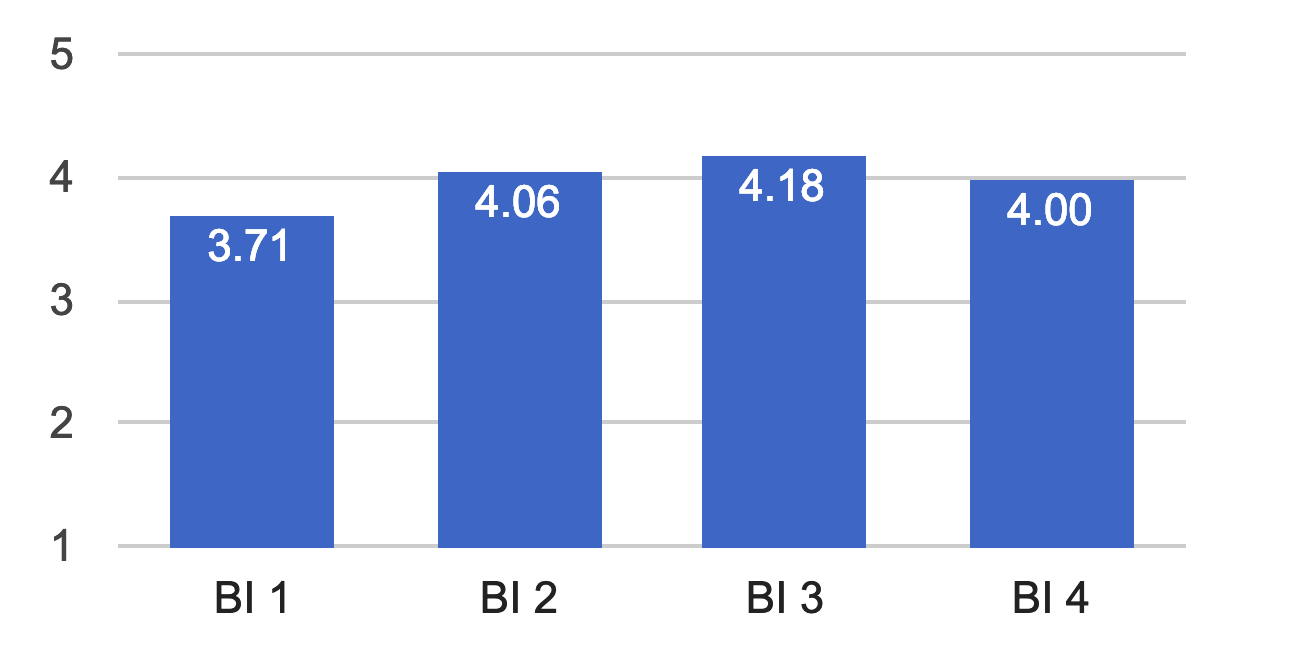
\includegraphics[width=9cm]{overall/bi.png}
		\captionof{figure}{Intention to use}
		 \label{fig:overall-bi}
	\end{minipage}
	\begin{minipage}{4.5cm}
		
		\begin{tabular}{p{1cm} p{3.5cm}}

\toprule
BI 1    &   Overall rating of the Application \\
BI 2	&   Future intention to use for regular purchases \\
BI 3	&   Future intention to use while  travelling abroad \\
BI 4	&   Intention to recommend to friends \\
\bottomrule

\end{tabular}
	\end{minipage}\hfill

\end{table}


\begin{table}[H]
	\begin{minipage}{9cm}
		\centering
		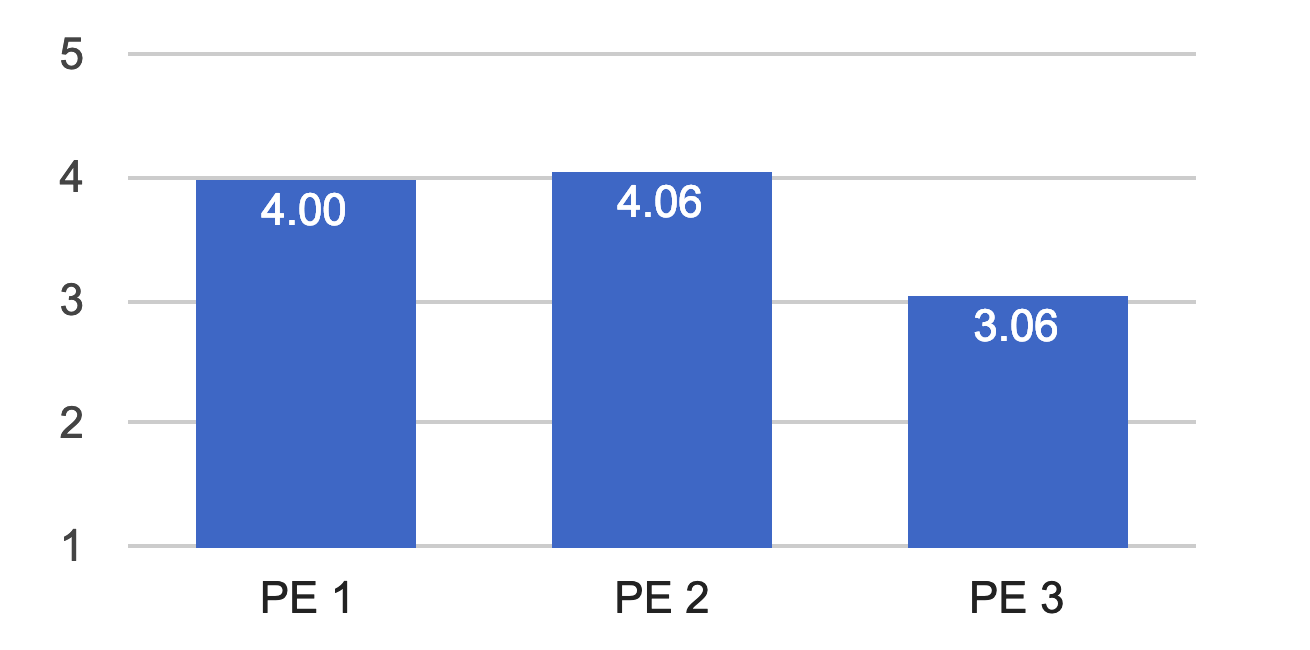
\includegraphics[width=9cm]{overall/pe.png}
		\captionof{figure}{Performance expectancy}
		 \label{fig:overall-pe}
	\end{minipage}
	\begin{minipage}{4.5cm}
		
		\begin{tabular}{p{1cm} p{3.5cm}}

\toprule
PE 1    &	Job-fit \\
PE 2    &	Relative advantage (Time-saving) \\
PE 3    &	Perceived usefulness \\
\bottomrule

\end{tabular}
	\end{minipage}\hfill

\end{table}


\begin{table}[H]
	\begin{minipage}{9cm}
		\centering
		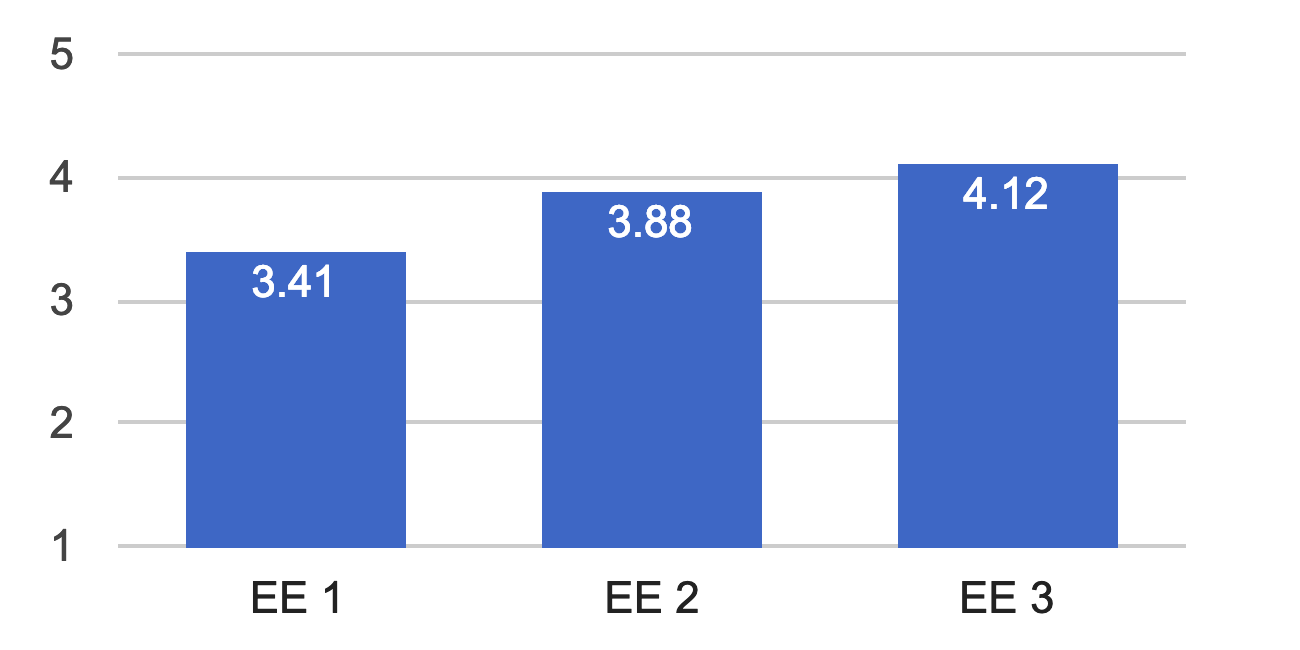
\includegraphics[width=9cm]{overall/ee.png}
		\captionof{figure}{Effort expectancy}
		 \label{fig:overall-ee}
	\end{minipage}
	\begin{minipage}{4.5cm}
		
		\begin{tabular}{p{1cm} p{3.5cm}}

\toprule
EE 1    &	Perceived ease of use \\
EE 2    &	Complexity \\
EE 3    &	Ease of use \\
\bottomrule

\end{tabular}
	\end{minipage}\hfill

\end{table}


\begin{table}[H]
\centering
\begin{tabular}{|c|c|c|c|}
\hline
Users & Days of usage & Products scanned & Products captured \\ \hline
16    & 4.56          & 18.06            & 1.88              \\ \hline
\end{tabular}
\caption{Overall usage data}
        \label{tab:usage-overall}
\end{table}


\newpage

\section{Tailoring}

    \begin{figure}[H]
      \centering
      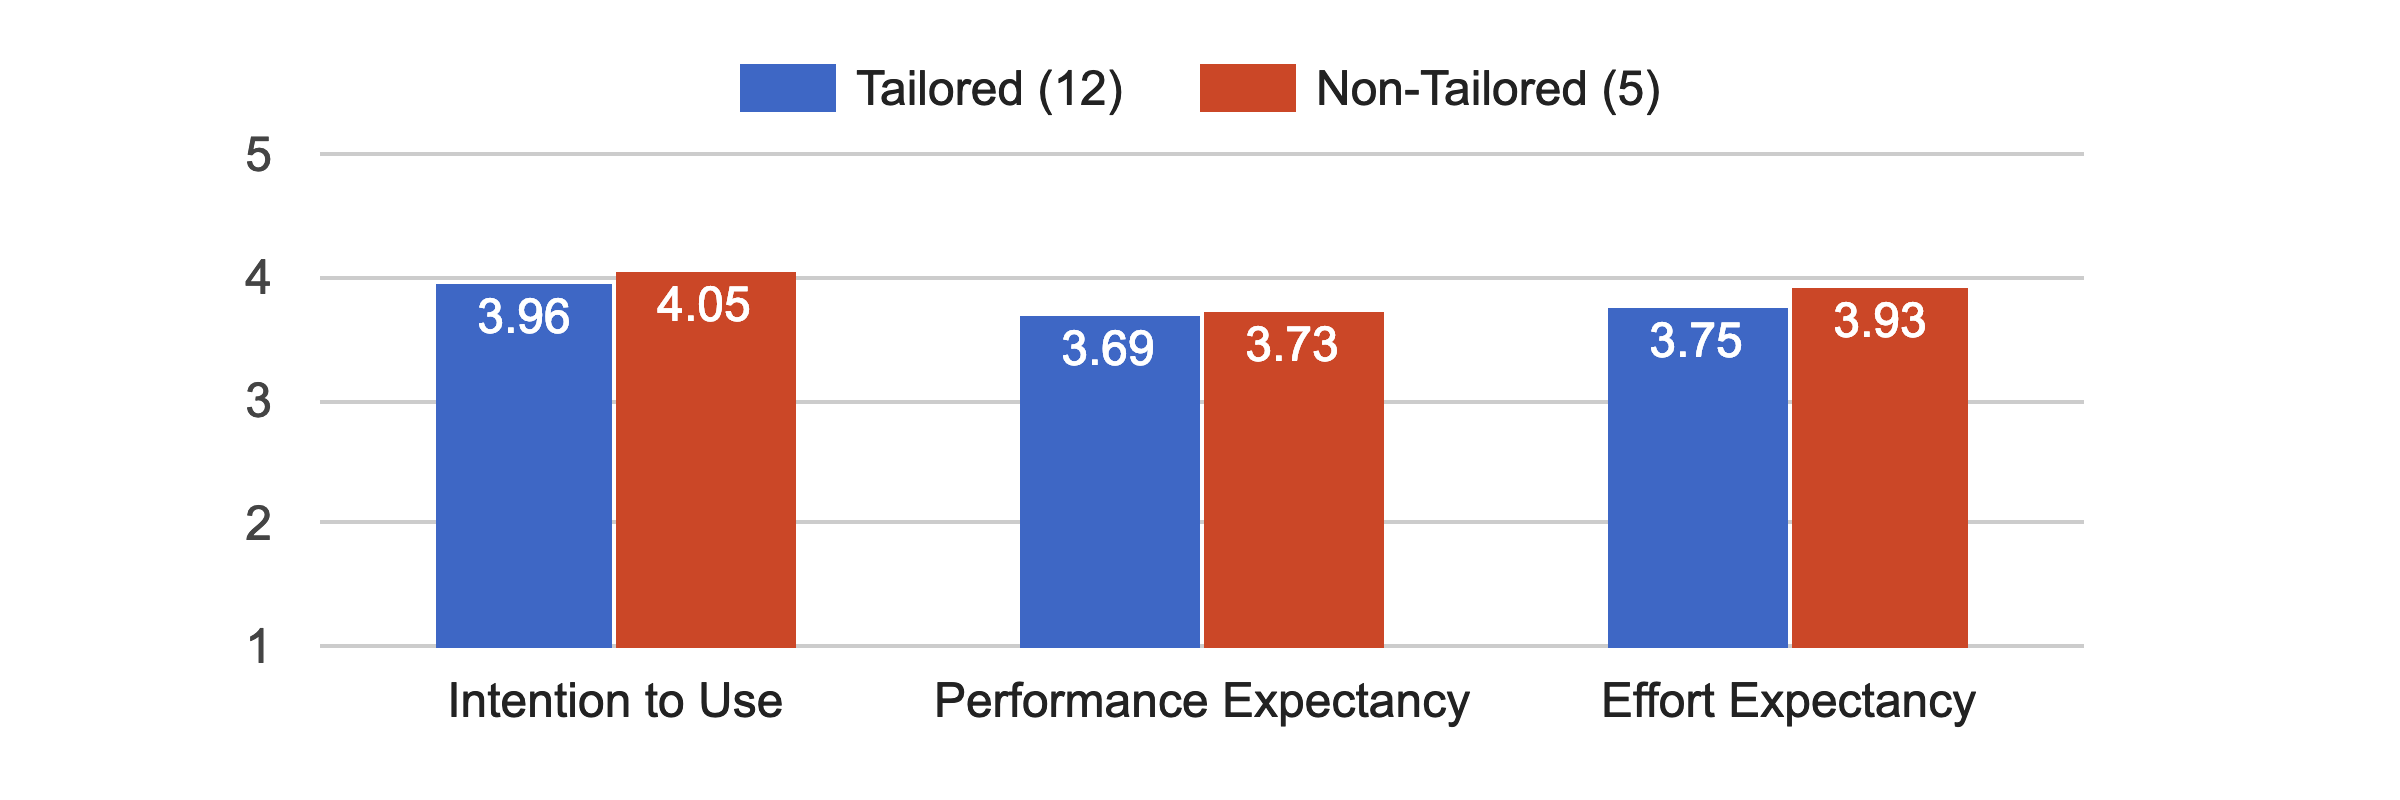
\includegraphics[width=\textwidth]{feedback/tailoring.png}
      \caption{Feedback by tailoring}
      \label{fig:feedback-tailoring}
      \end{figure}
      
    \begin{table}[H]
        \begin{tabular}{l|c|c|c|c|}
        \cline{2-5}
            & Users & Days of usage & Products scanned & Products captured \\ \hline
            \multicolumn{1}{|l|}{\textbf{Tailored}}     & 11          & 3.55          & 15.09            & 1.36              \\ \hline
            \multicolumn{1}{|l|}{\textbf{Non-Tailored}} & 5           & 6.80          & 24.60            & 3.00              \\ \hline
        \end{tabular}
        \caption{Usage data by tailoring}
        \label{tab:usage-tailoring}
    \end{table}

\section{Visualization}

    \begin{figure}[H]
      \centering
      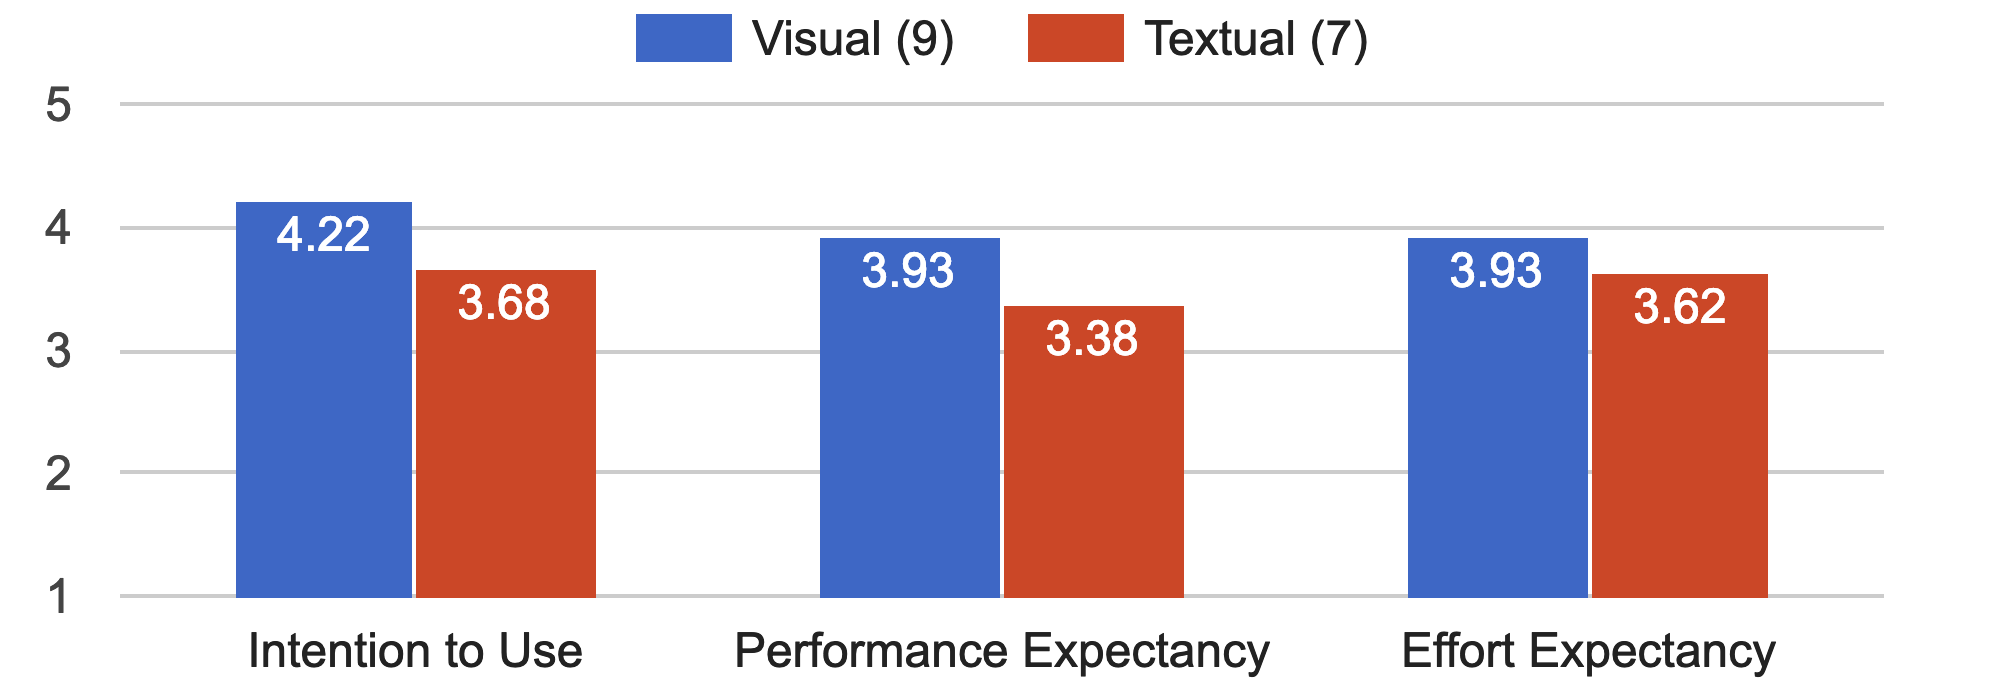
\includegraphics[width=\textwidth]{feedback/presentation.png}
      \caption{Feedback by visualization}
      \label{fig:feedback-presentation}
      \end{figure}
      
    \begin{table}[H]
        \begin{tabular}{l|c|c|c|c|}
        \cline{2-5}
            & Users & Days of usage & Products scanned & Products captured \\ \hline
            \multicolumn{1}{|l|}{\textbf{Visual}}     & 9          & 3.67	          & 16.00        & 0.11              \\ \hline
            \multicolumn{1}{|l|}{\textbf{Textual}} & 7           & 5.71          & 20.71            & 4.14              \\ \hline
        \end{tabular}
        \caption{Usage data by visualization}
        \label{tab:usage-presentation}
    \end{table}

\section{Gender}

    \begin{figure}[H]
      \centering
      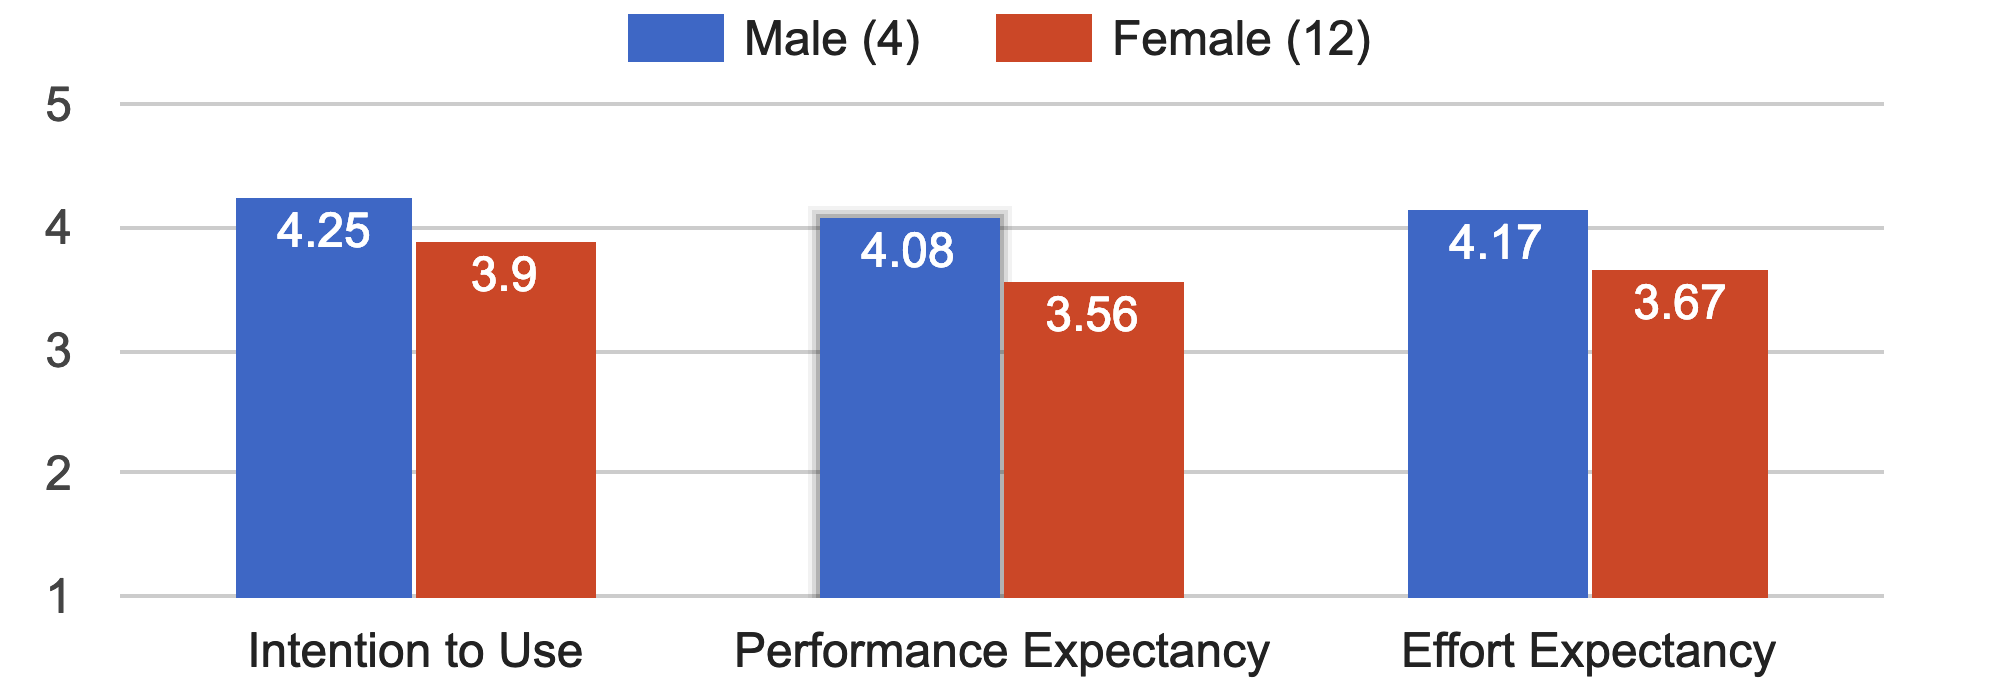
\includegraphics[width=\textwidth]{feedback/gender.png}
      \caption{Feedback by gender}
      \label{fig:feedback-gender}
      \end{figure}
      
    \begin{table}[H]
        \begin{tabular}{l|c|c|c|c|}
        \cline{2-5}
            & Users & Days of usage & Products scanned & Products captured \\ \hline
            \multicolumn{1}{|l|}{\textbf{Male}}     & 4          & 7.75          & 29.50            & 6.00              \\ \hline
            \multicolumn{1}{|l|}{\textbf{Female}} & 12           & 3.50          & 14.25            & 0.50              \\ \hline
        \end{tabular}
        \caption{Usage data by gender}
        \label{tab:usage-gender}
    \end{table}

\section{Age}

    \begin{figure}[H]
      \centering
      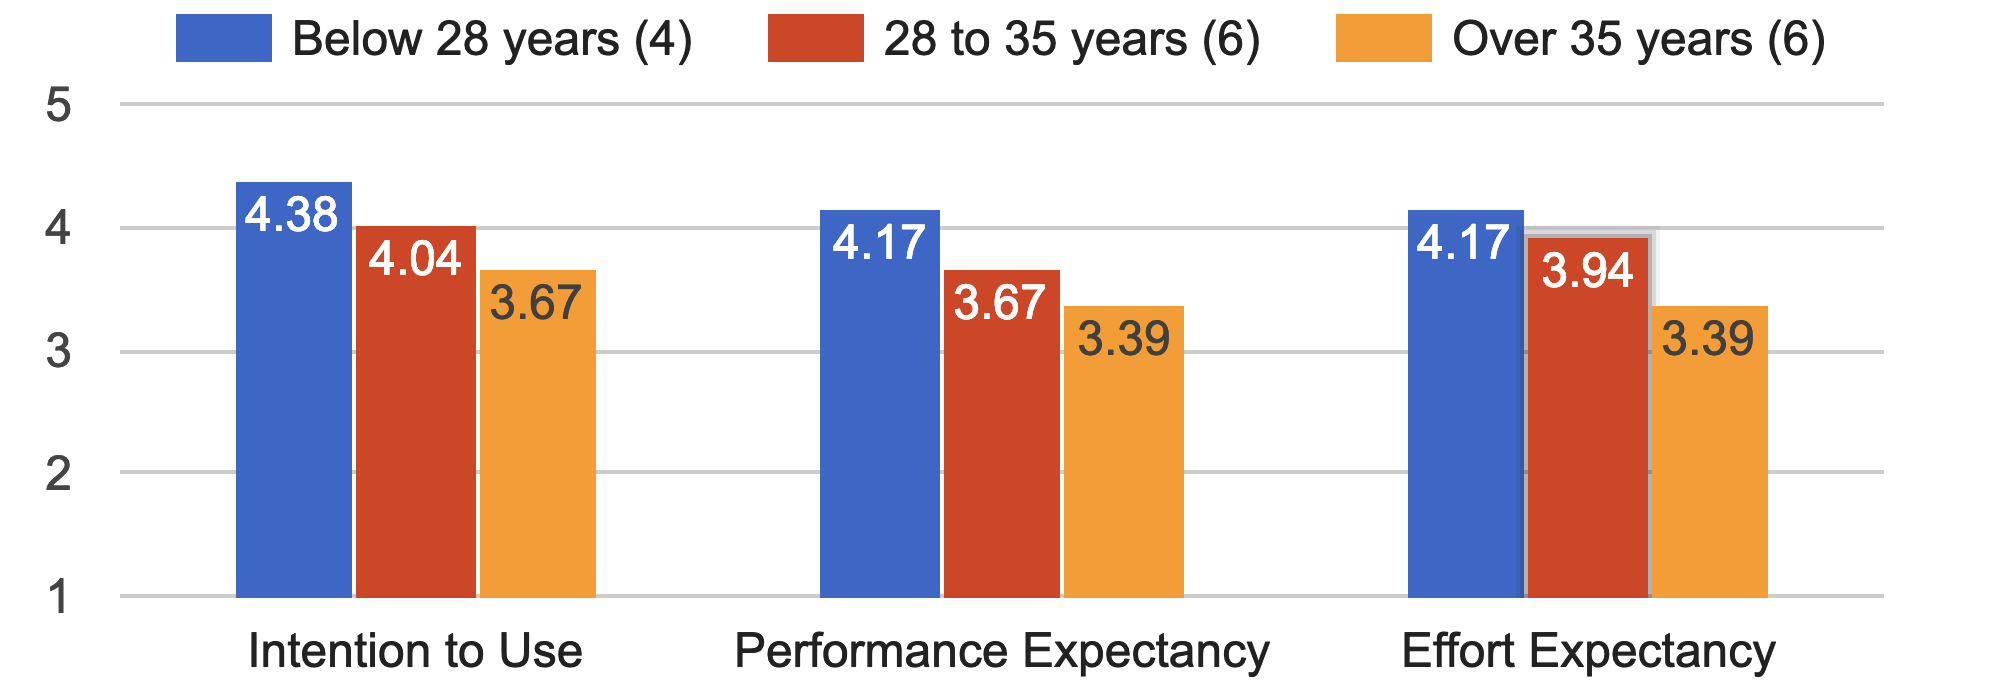
\includegraphics[width=\textwidth]{feedback/age.png}
      \caption{Feedback by age}
      \label{fig:feedback-age}
      \end{figure}
      
    \begin{table}[H]
        \begin{tabular}{l|c|c|c|c|}
        \cline{2-5}
            & Users & Days of usage & Products scanned & Products captured \\ \hline
            \multicolumn{1}{|l|}{\textbf{Below 28 years}}     & 4          & 5.25          & 14.50            & 1.50              \\ \hline
            \multicolumn{1}{|l|}{\textbf{28 to 35 years}} & 6           & 4.67          & 18.17            & 1.50              \\ \hline
            \multicolumn{1}{|l|}{\textbf{Over 35 years}} & 6           & 4.00          & 20.33            & 2.50              \\ \hline
        \end{tabular}
        \caption{Usage data by age}
        \label{tab:usage-age}
    \end{table}

\section{Travel Frequency}

    \begin{figure}[H]
      \centering
      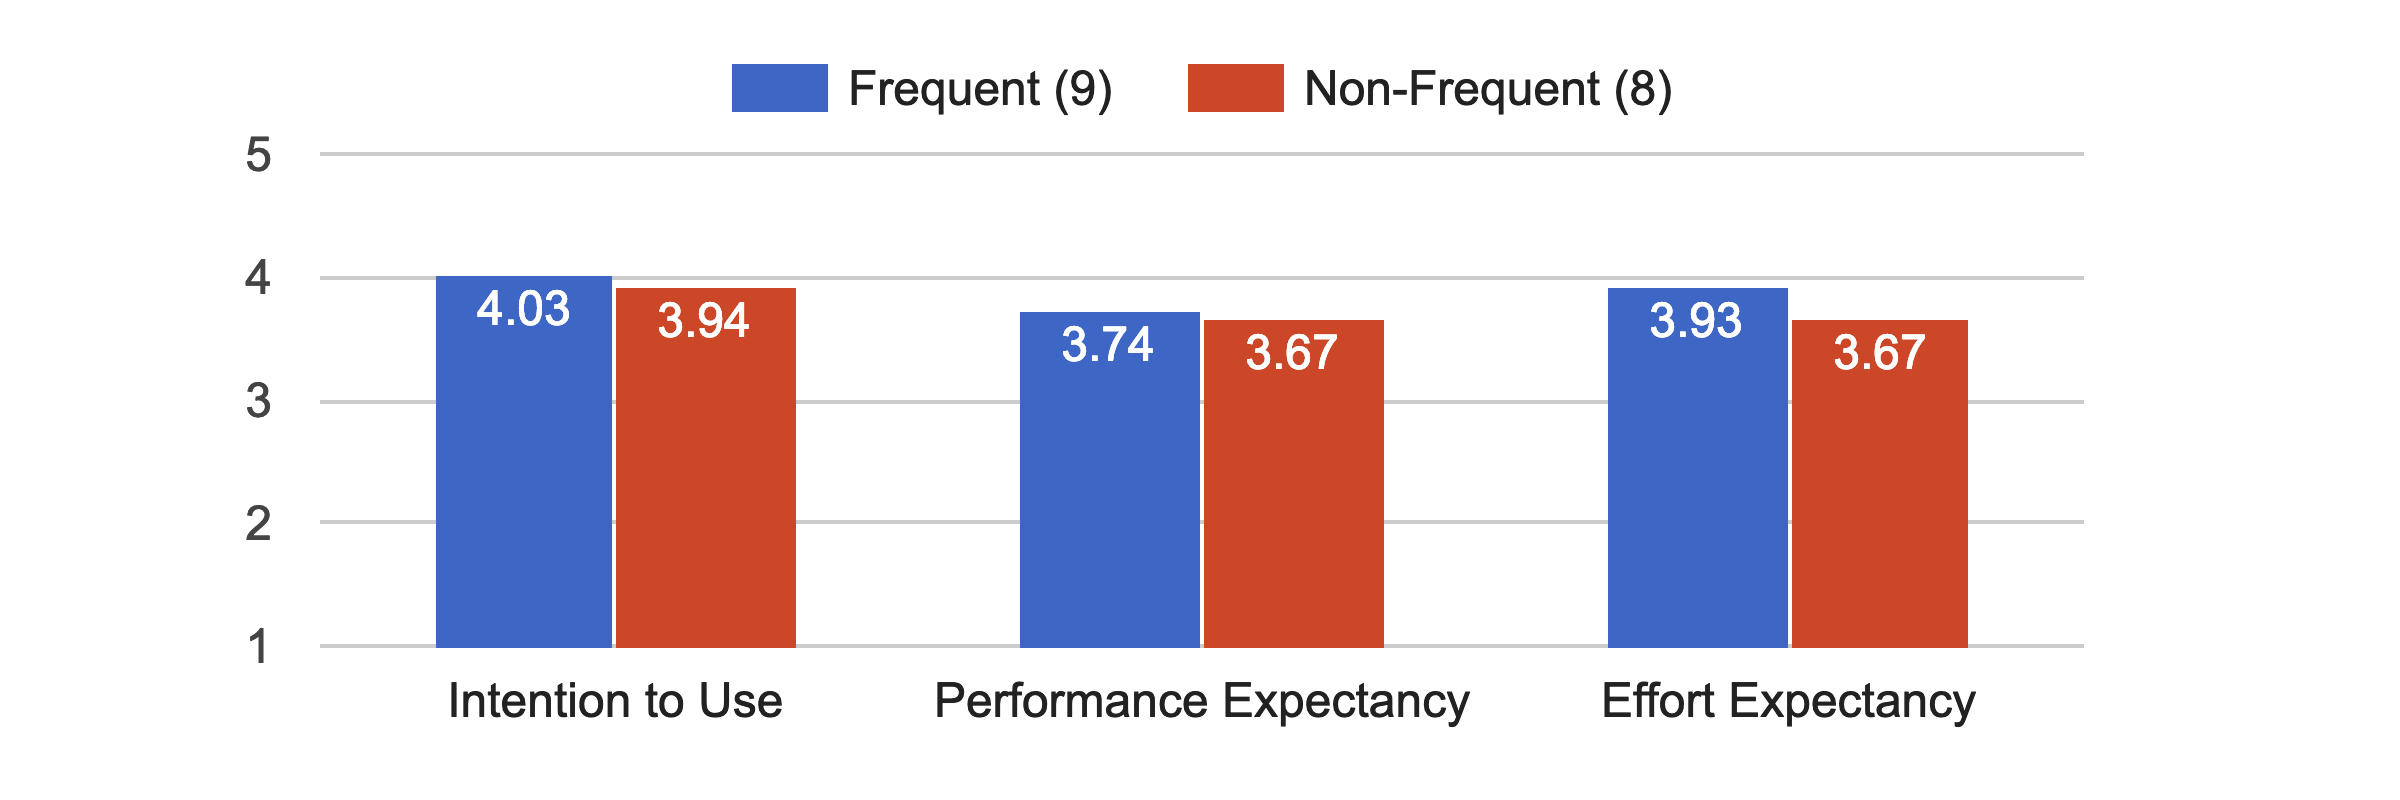
\includegraphics[width=\textwidth]{feedback/travelling.png}
      \caption{Feedback by travel frequency}
      \label{fig:feedback-travelling}
      \end{figure}
      
    \begin{table}[H]
        \begin{tabular}{l|c|c|c|c|}
        \cline{2-5}
            & Users & Days of usage & Products scanned & Products captured \\ \hline
            \multicolumn{1}{|l|}{\textbf{Frequent}}     & 8          & 4.38          & 18.50            & 1.13              \\ \hline
            \multicolumn{1}{|l|}{\textbf{Non-Frequent}} & 8           & 4.75          & 17.63            & 2.63              \\ \hline
        \end{tabular}
        \caption{Usage data by travel frequency}
        \label{tab:usage-travelling}
    \end{table}

\section{German Language Level}

    \begin{figure}[H]
      \centering
      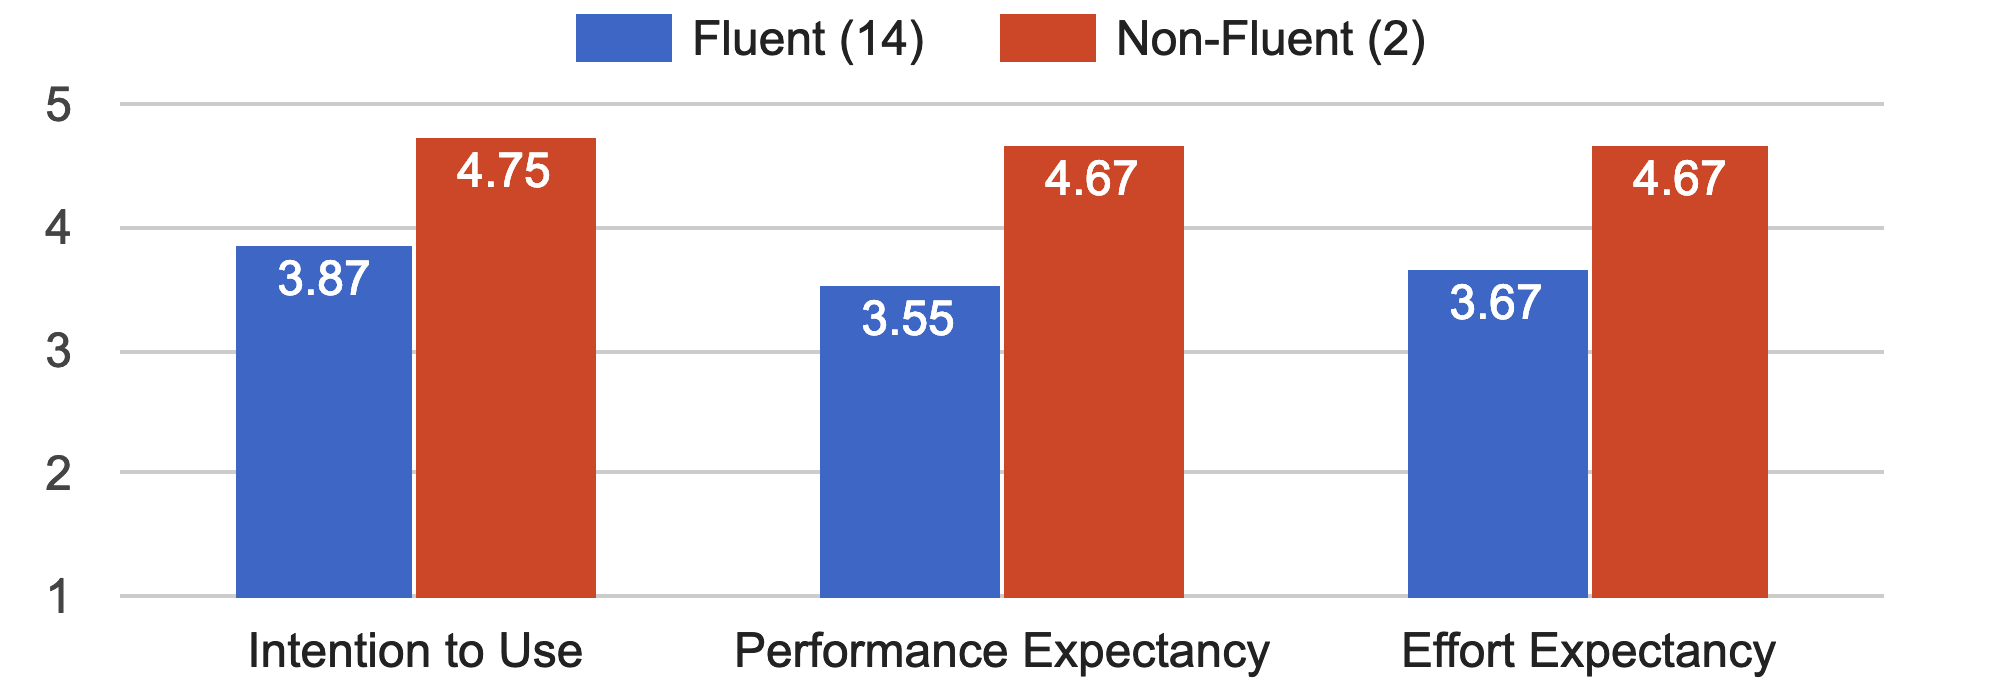
\includegraphics[width=\textwidth]{feedback/german.png}
      \caption{Feedback by German language level}
      \label{fig:feedback-german}
      \end{figure}
      
    \begin{table}[H]
        \begin{tabular}{l|c|c|c|c|}
        \cline{2-5}
            & Users & Days of usage & Products scanned & Products captured \\ \hline
            \multicolumn{1}{|l|}{\textbf{Fluent}}     & 14          & 4.79          & 19.43            & 2.14              \\ \hline
            \multicolumn{1}{|l|}{\textbf{Non-Fluent}} & 2           & 3.00          & 8.50            & 0.00              \\ \hline
        \end{tabular}
        \caption{Usage data by German language level}
        \label{tab:usage-german}
    \end{table}

\section{Device Language}

    \begin{figure}[H]
      \centering
      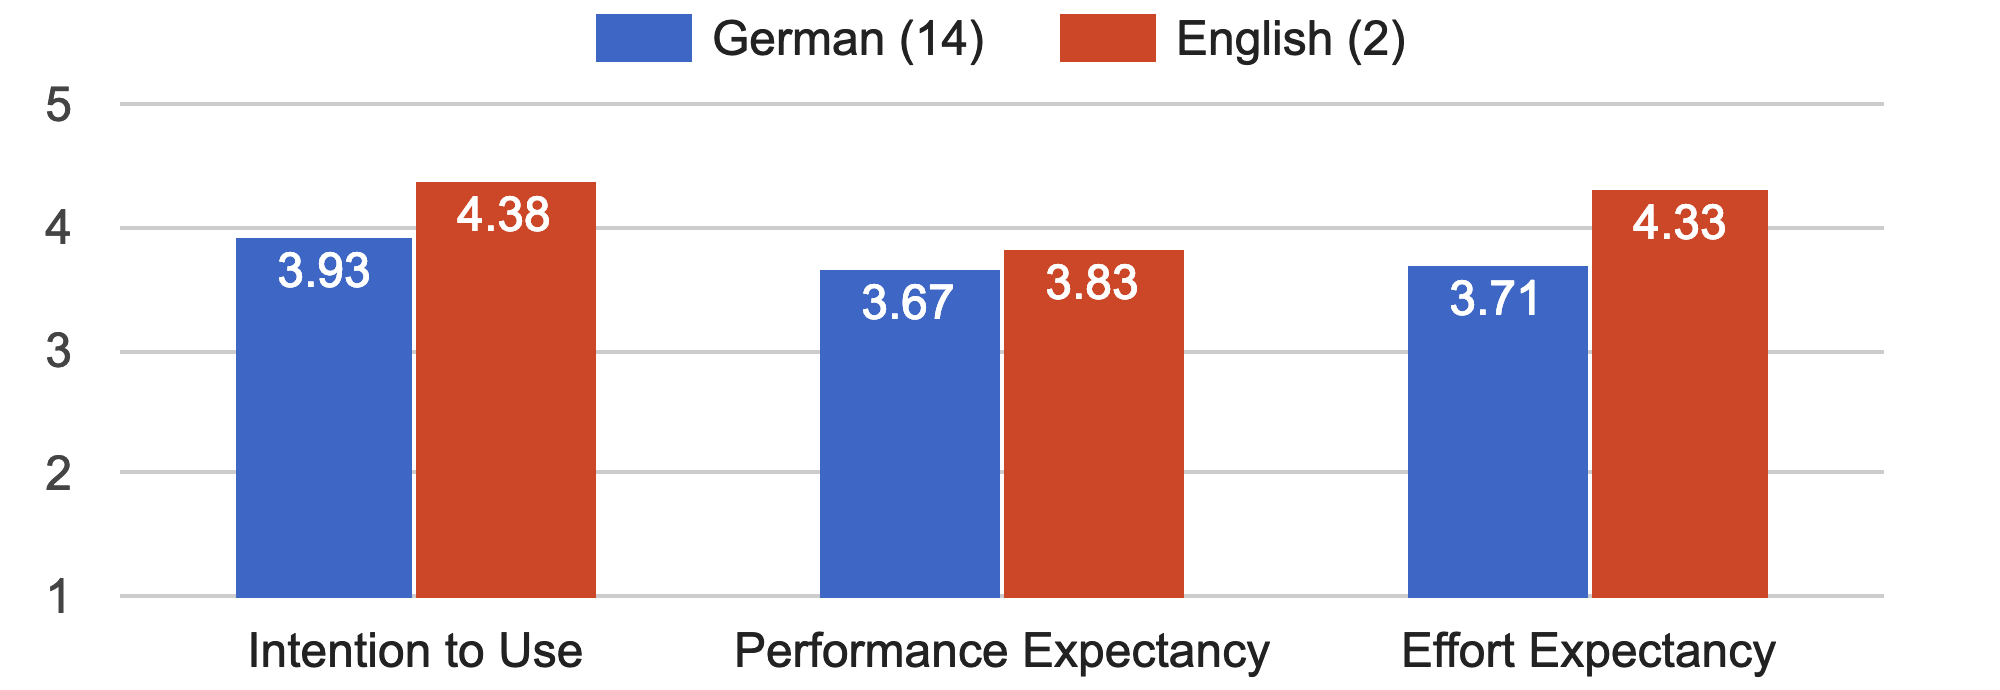
\includegraphics[width=\textwidth]{feedback/lang.png}
      \caption{Feedback by device language}
      \label{fig:feedback-lang}
      \end{figure}
      
    \begin{table}[H]
        \begin{tabular}{l|c|c|c|c|}
        \cline{2-5}
            & Users & Days of usage & Products scanned & Products captured \\ \hline
            \multicolumn{1}{|l|}{\textbf{German}}     & 14          & 4.36          & 17.57            & 1.57              \\ \hline
            \multicolumn{1}{|l|}{\textbf{English}} & 2           & 6.00          & 21.50            & 4.00              \\ \hline
        \end{tabular}
        \caption{Usage data by device language}
        \label{tab:usage-lang}
    \end{table}
    
\section{Amount of Allergies}

    \begin{figure}[H]
      \centering
      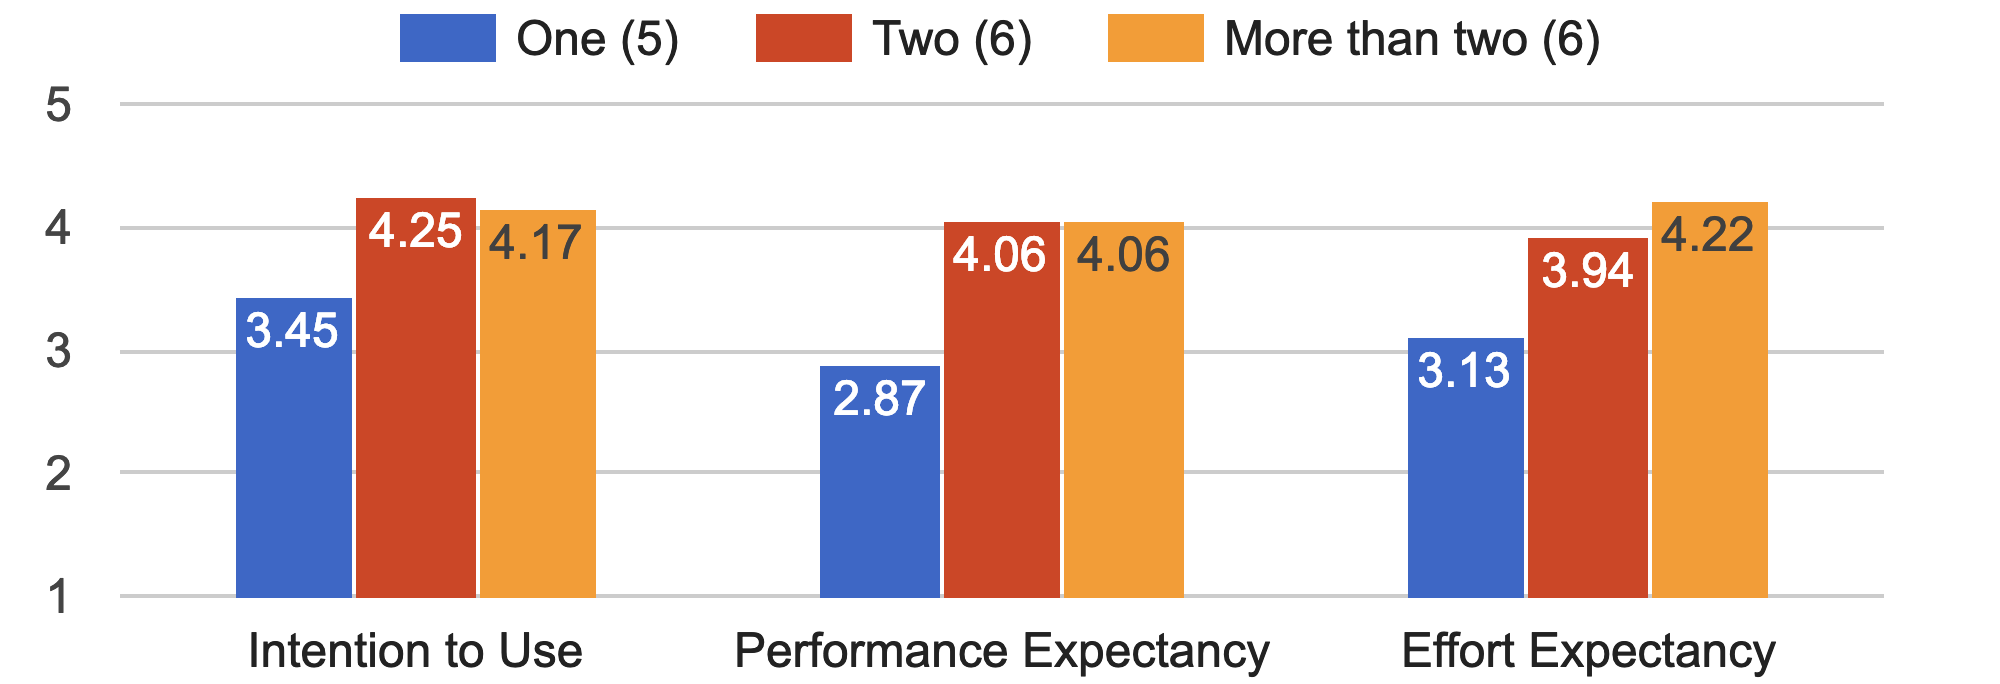
\includegraphics[width=\textwidth]{feedback/allergies.png}
      \caption{Feedback by amounts of allergies}
      \label{fig:feedback-allergies}
      \end{figure}
      
    \begin{table}[H]
        \begin{tabular}{l|c|c|c|c|}
        \cline{2-5}
            & Users & Days of usage & Products scanned & Products captured \\ \hline
            \multicolumn{1}{|l|}{\textbf{One}}     & 5          & 3.60          & 16.60            & 0.20              \\ \hline
            \multicolumn{1}{|l|}{\textbf{Two}}     & 6          & 3.50          & 13.17            & 2.33              \\ \hline
            \multicolumn{1}{|l|}{\textbf{More than two}} & 5           & 6.80          & 25.40            & 3.00              \\ \hline
        \end{tabular}
        \caption{Usage data by amounts of allergies}
        \label{tab:usage-allergies}
    \end{table}

\section{Successful Scans Ratio}

    \begin{figure}[H]
      \centering
      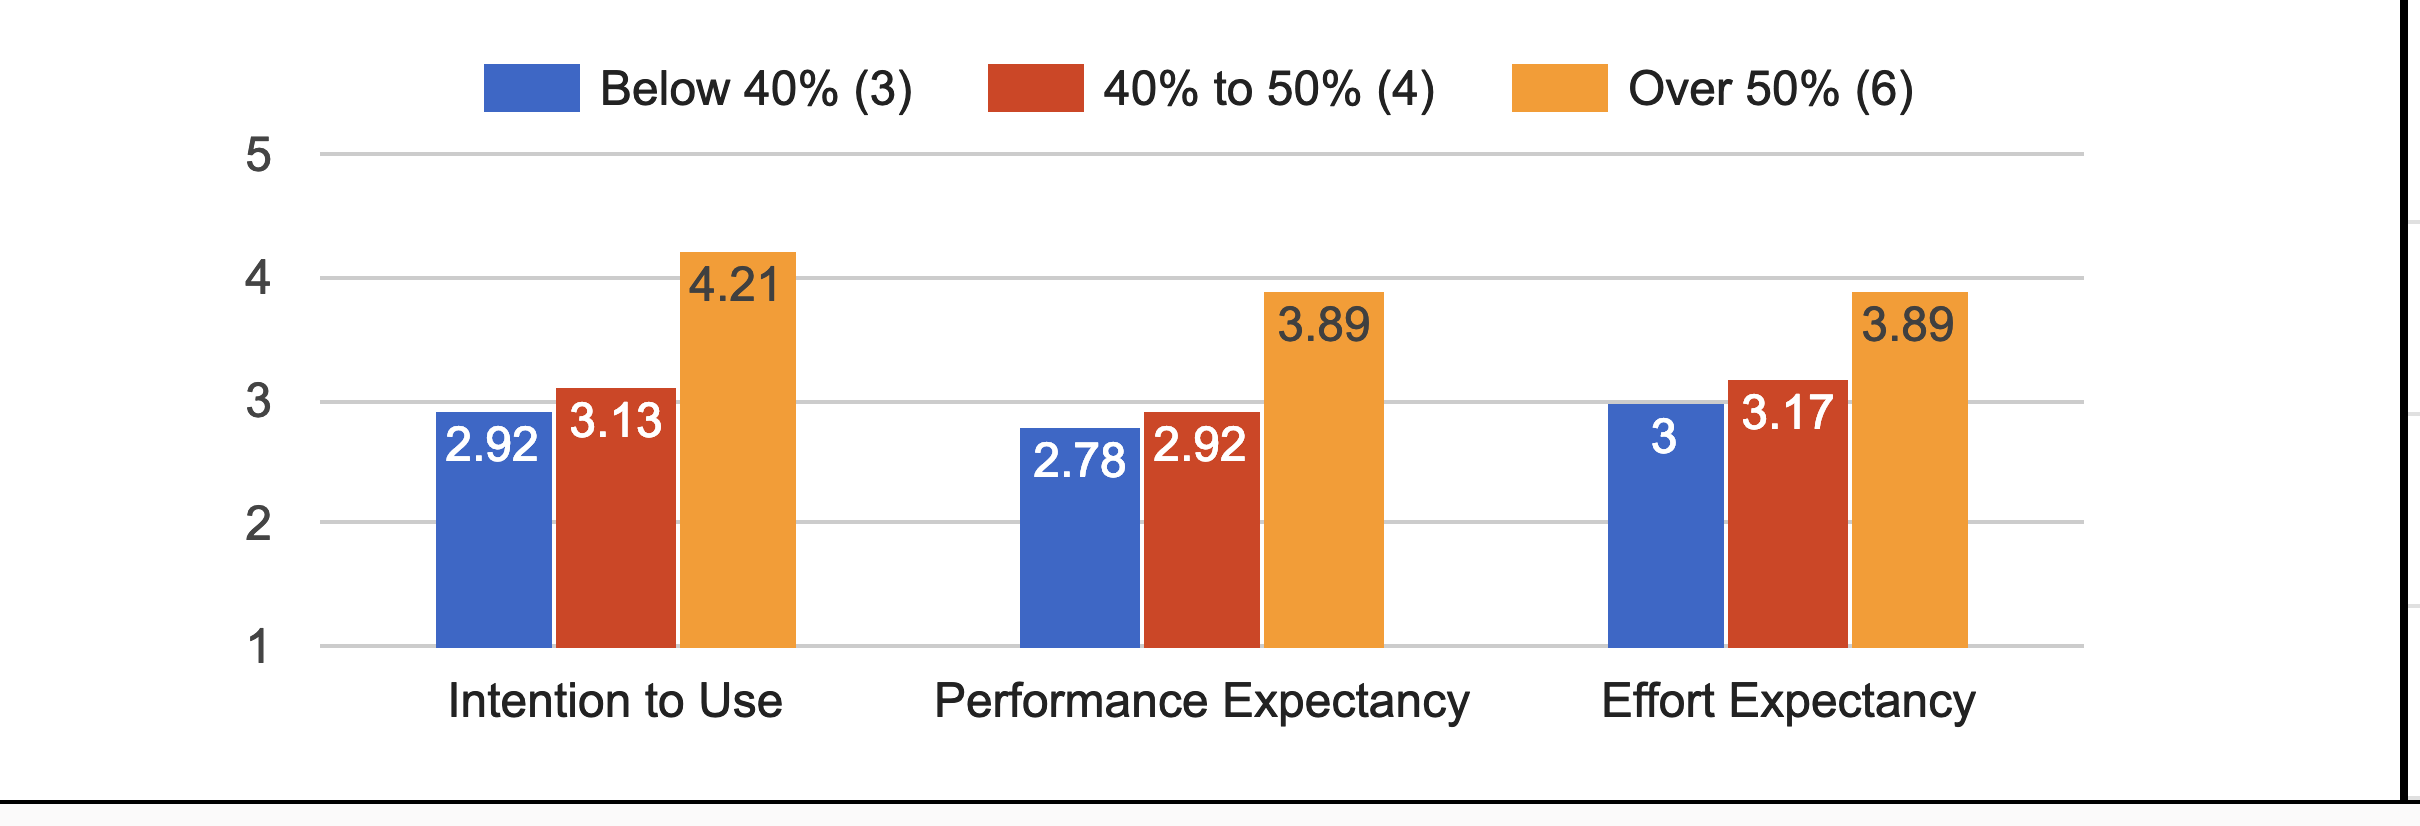
\includegraphics[width=\textwidth]{feedback/ratio.png}
      \caption{Feedback by successful scans ratio}
      \label{fig:feedback-ratio}
      \end{figure}
      
    \begin{table}[H]
        \begin{tabular}{l|c|c|c|c|}
        \cline{2-5}
            & Users & Days of usage & Products scanned & Products captured \\ \hline
            \multicolumn{1}{|l|}{\textbf{Below 40\%}}     & 5          & 4.60          & 20.20            & 2.40              \\ \hline
            \multicolumn{1}{|l|}{\textbf{40\% to 50\%}}     & 6          & 6.00          & 24.83            & 2.33              \\ \hline
            \multicolumn{1}{|l|}{\textbf{Over 50\%}} & 5           & 2.80          & 7.80            & 0.80              \\ \hline
        \end{tabular}
        \caption{Usage data by successful scans ratio}
        \label{tab:usage-ratio}
    \end{table}

\section{Allergy Awareness}

    \begin{figure}[H]
      \centering
      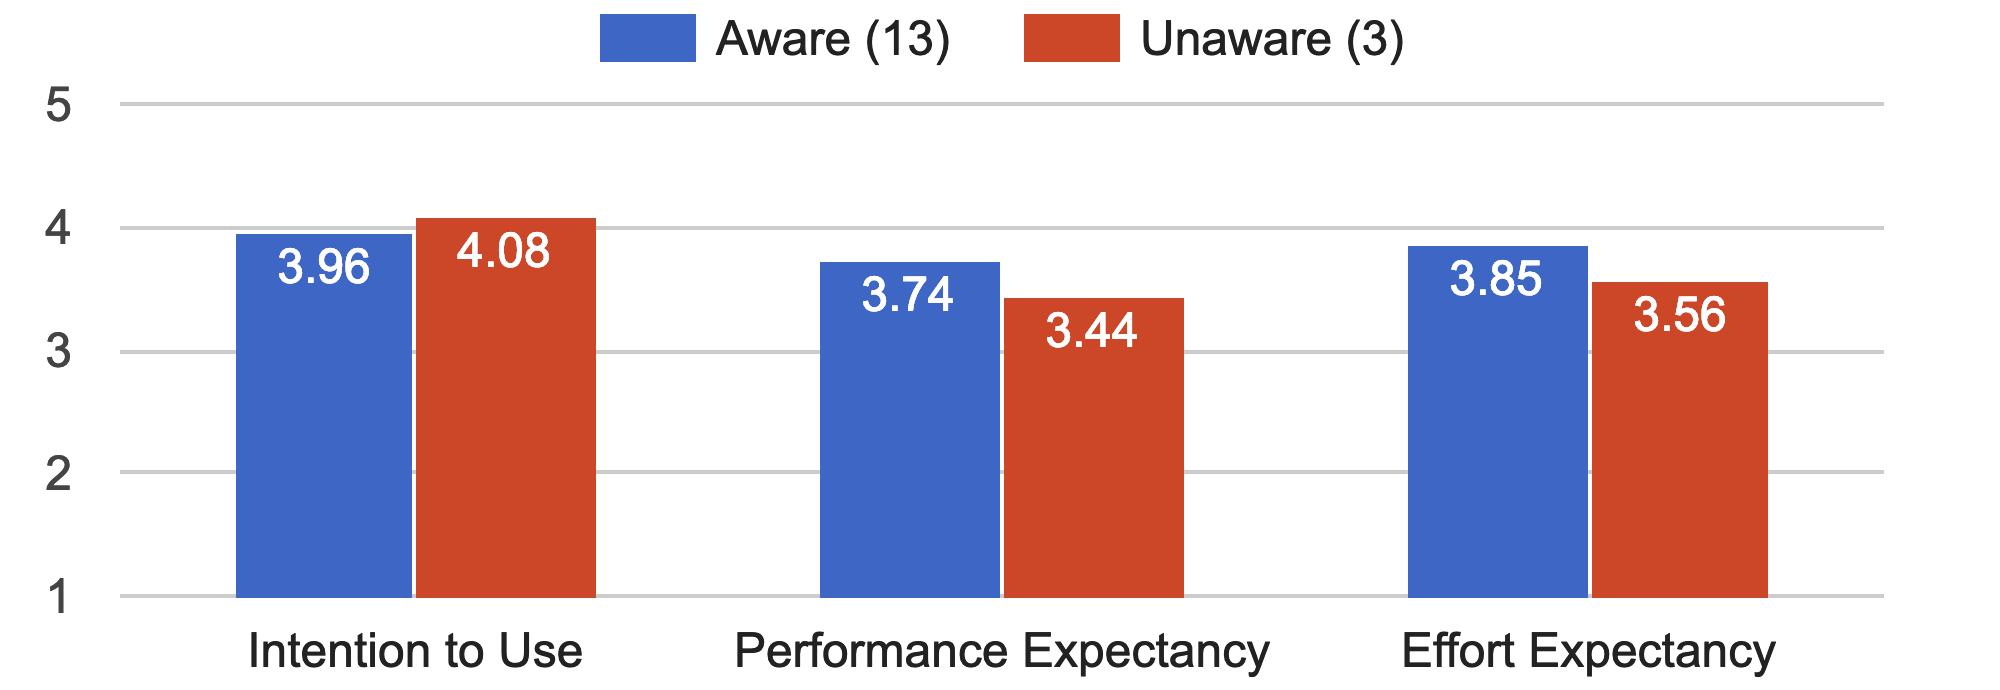
\includegraphics[width=\textwidth]{feedback/research.png}
      \caption{Feedback by allergy awareness}
      \label{fig:feedback-research}
      \end{figure}
      
    \begin{table}[H]
        \begin{tabular}{l|c|c|c|c|}
        \cline{2-5}
            & Users & Days of usage & Products scanned & Products captured \\ \hline
            \multicolumn{1}{|l|}{\textbf{Aware}}     & 13          & 4.77          & 20.00            & 2.00              \\ \hline
            \multicolumn{1}{|l|}{\textbf{Unaware}}     & 3          & 3.67          & 9.67            & 1.33              \\ \hline
        \end{tabular}
        \caption{Usage data by allergy awareness}
        \label{tab:usage-research}
    \end{table}